\section{Higgs boson phenomenology}
%%%%%%%%%%%%%%%%%%%%%%%%%%%%%%%%%%%%%%%%%%%%%%%%%%%%%%%%%%%%%%%%%%%%%%
\label{sec:HiggsPheno}

In this section the Higgs boson production modes and decay channels are described, spending some time on the description of the \hww channel, which is the channel considered in this work. Afterwards, a brief review of the Monte Carlo (MC) generators used for the simulation of Higgs boson processes is given. Finally, a description of the effects due to higher order QCD corrections on variables like the Higgs boson transverse momentum are shown.

%One of the main goals of the LHC was the search for the SM Higgs boson over a wide range of masses. This goal has been achieved in 2012, when the ATLAS and CMS collaborations announced the discovery of a new boson with mass $m_\mathrm{H} = 125$\GeV~\cite{Aad:2012tfa,Chatrchyan:2012xdj}, consistent with the SM Higgs boson prediction.

%%%%%%%%%%%%%%%%%%%%%%%%%%%%%%%%%%%%%%%%%%%%%%%%%%%%%%%%%%%%%%%%%%%%%%
\subsection{Higgs boson production mechanisms and decay channels}

The main processes contributing to the Higgs boson production at hadron colliders are represented by the Feynman diagrams shown in Fig.~\ref{fig:higgs_prod}.

\begin{figure}[htb]
\centering
\subfigure[ggH]{
  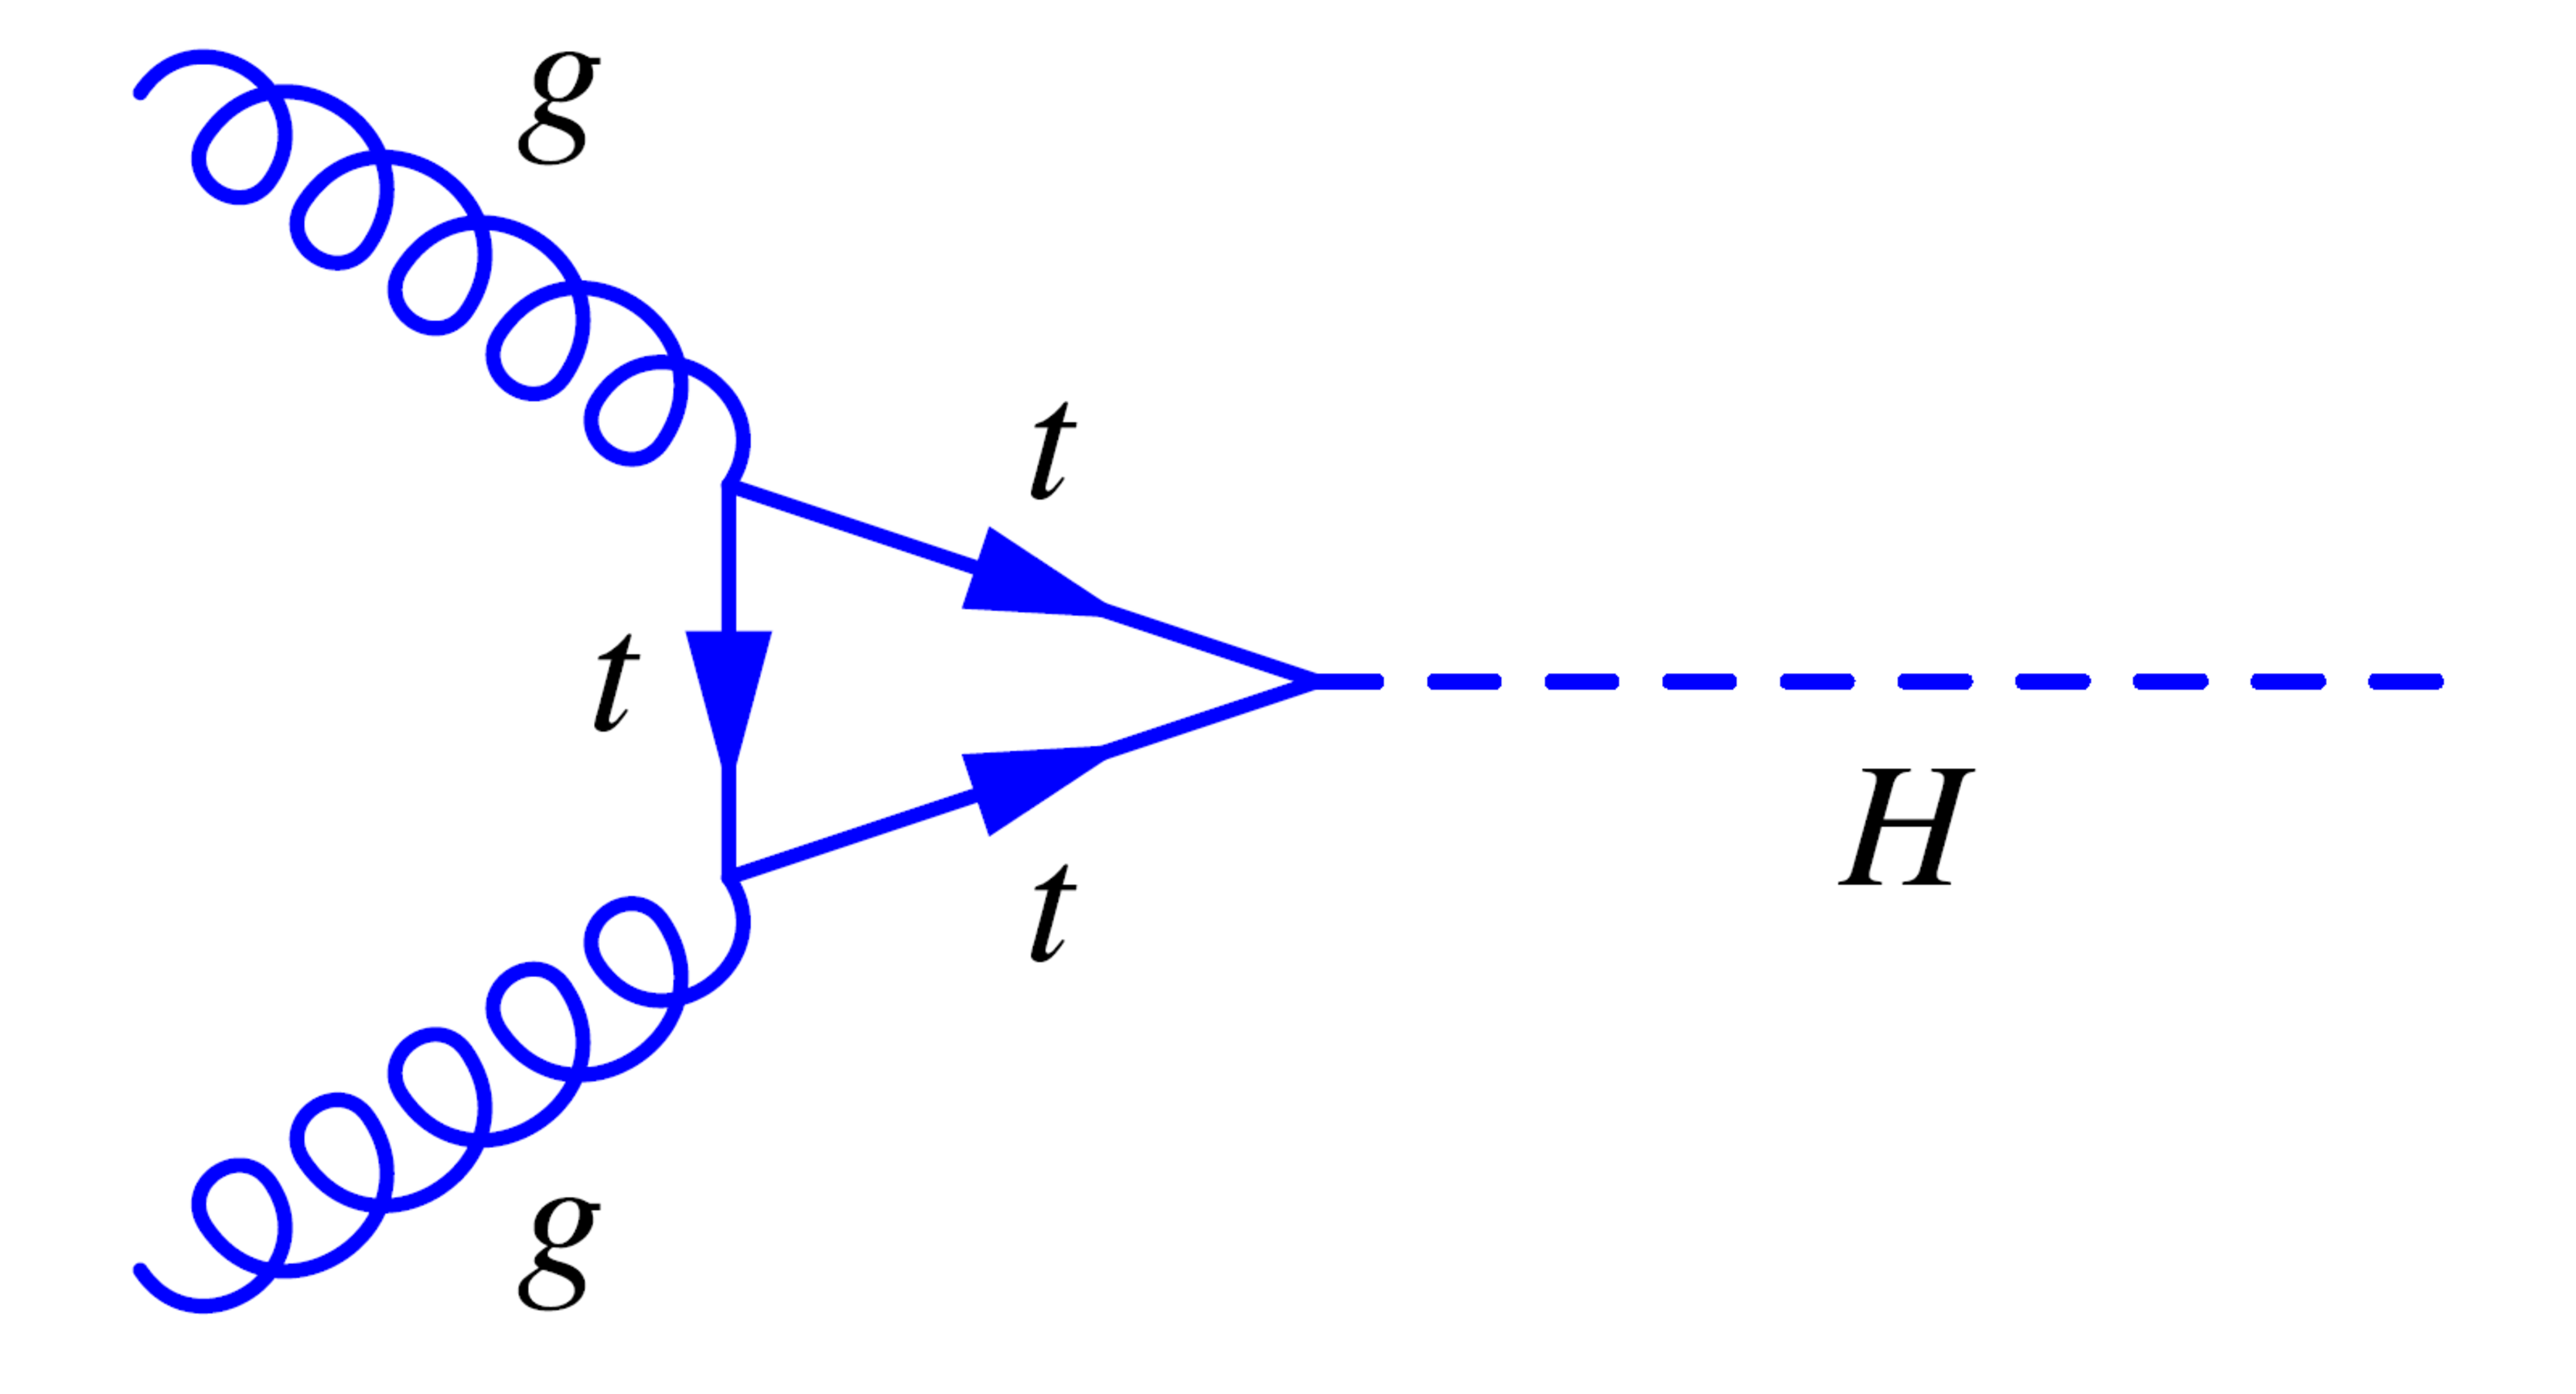
\includegraphics[width=0.45\textwidth]{images/ggH.pdf}
}
\subfigure[VBF]{
  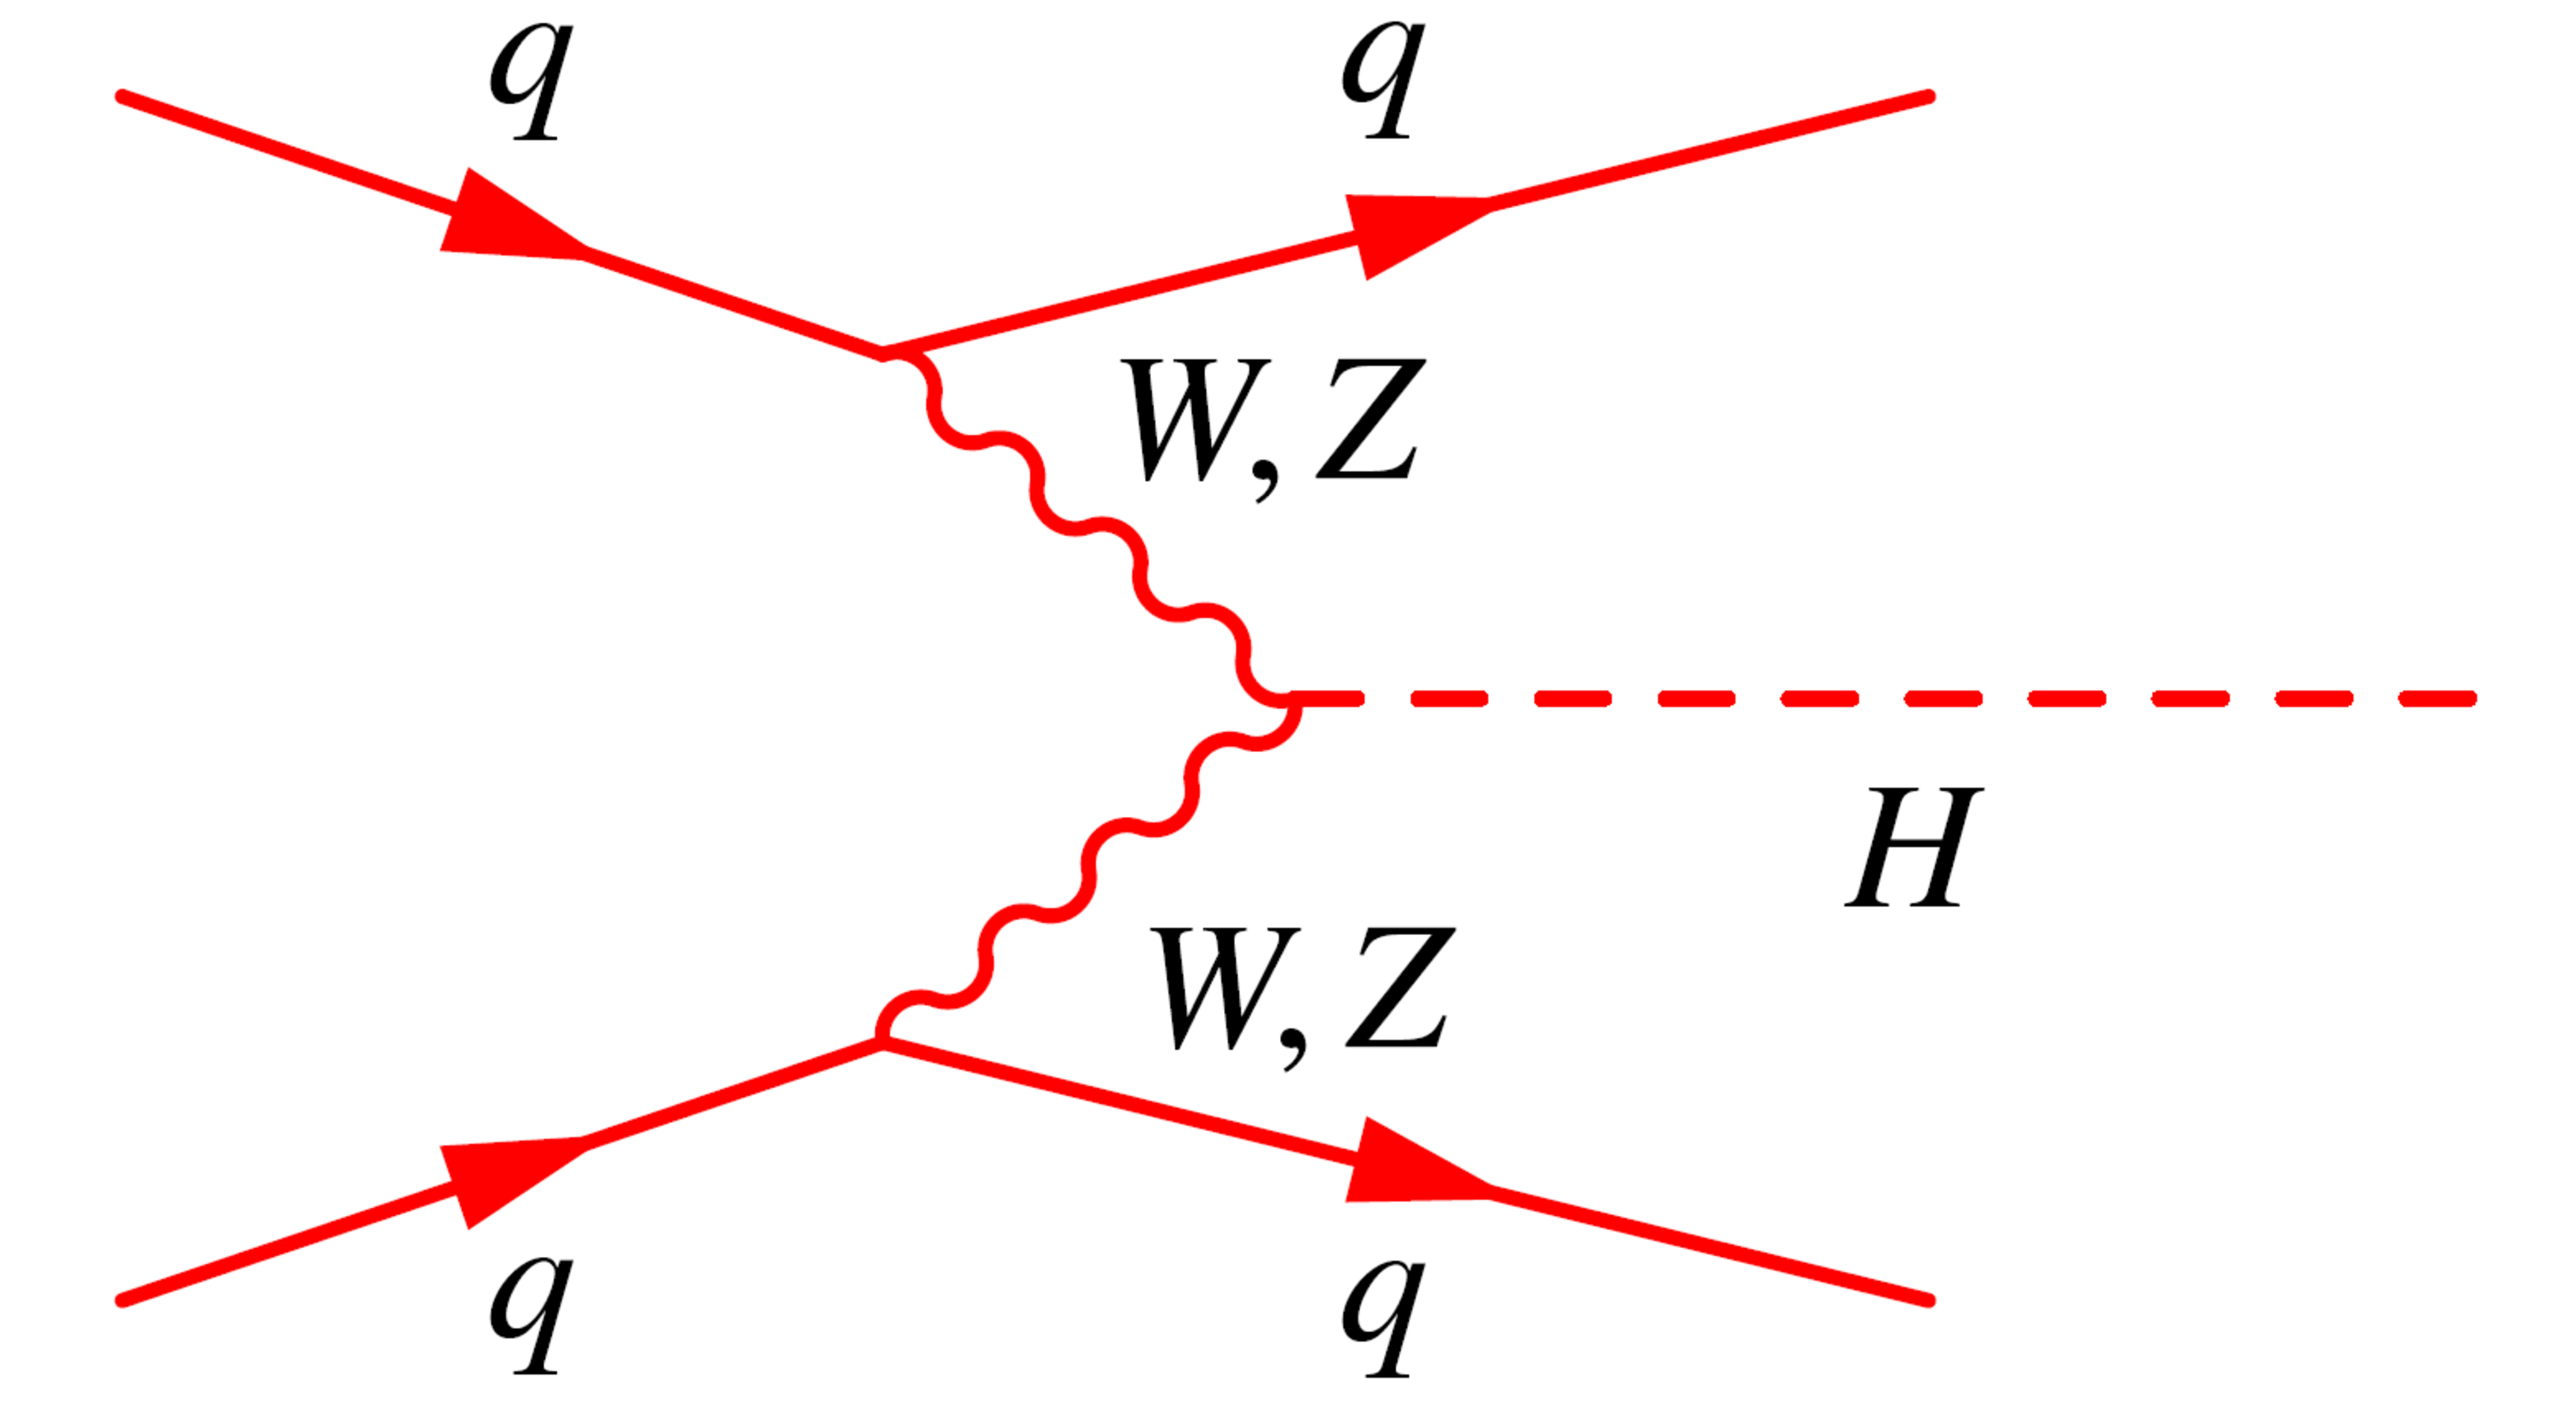
\includegraphics[width=0.45\textwidth]{images/VBF.pdf}
}\\
\subfigure[VH]{
  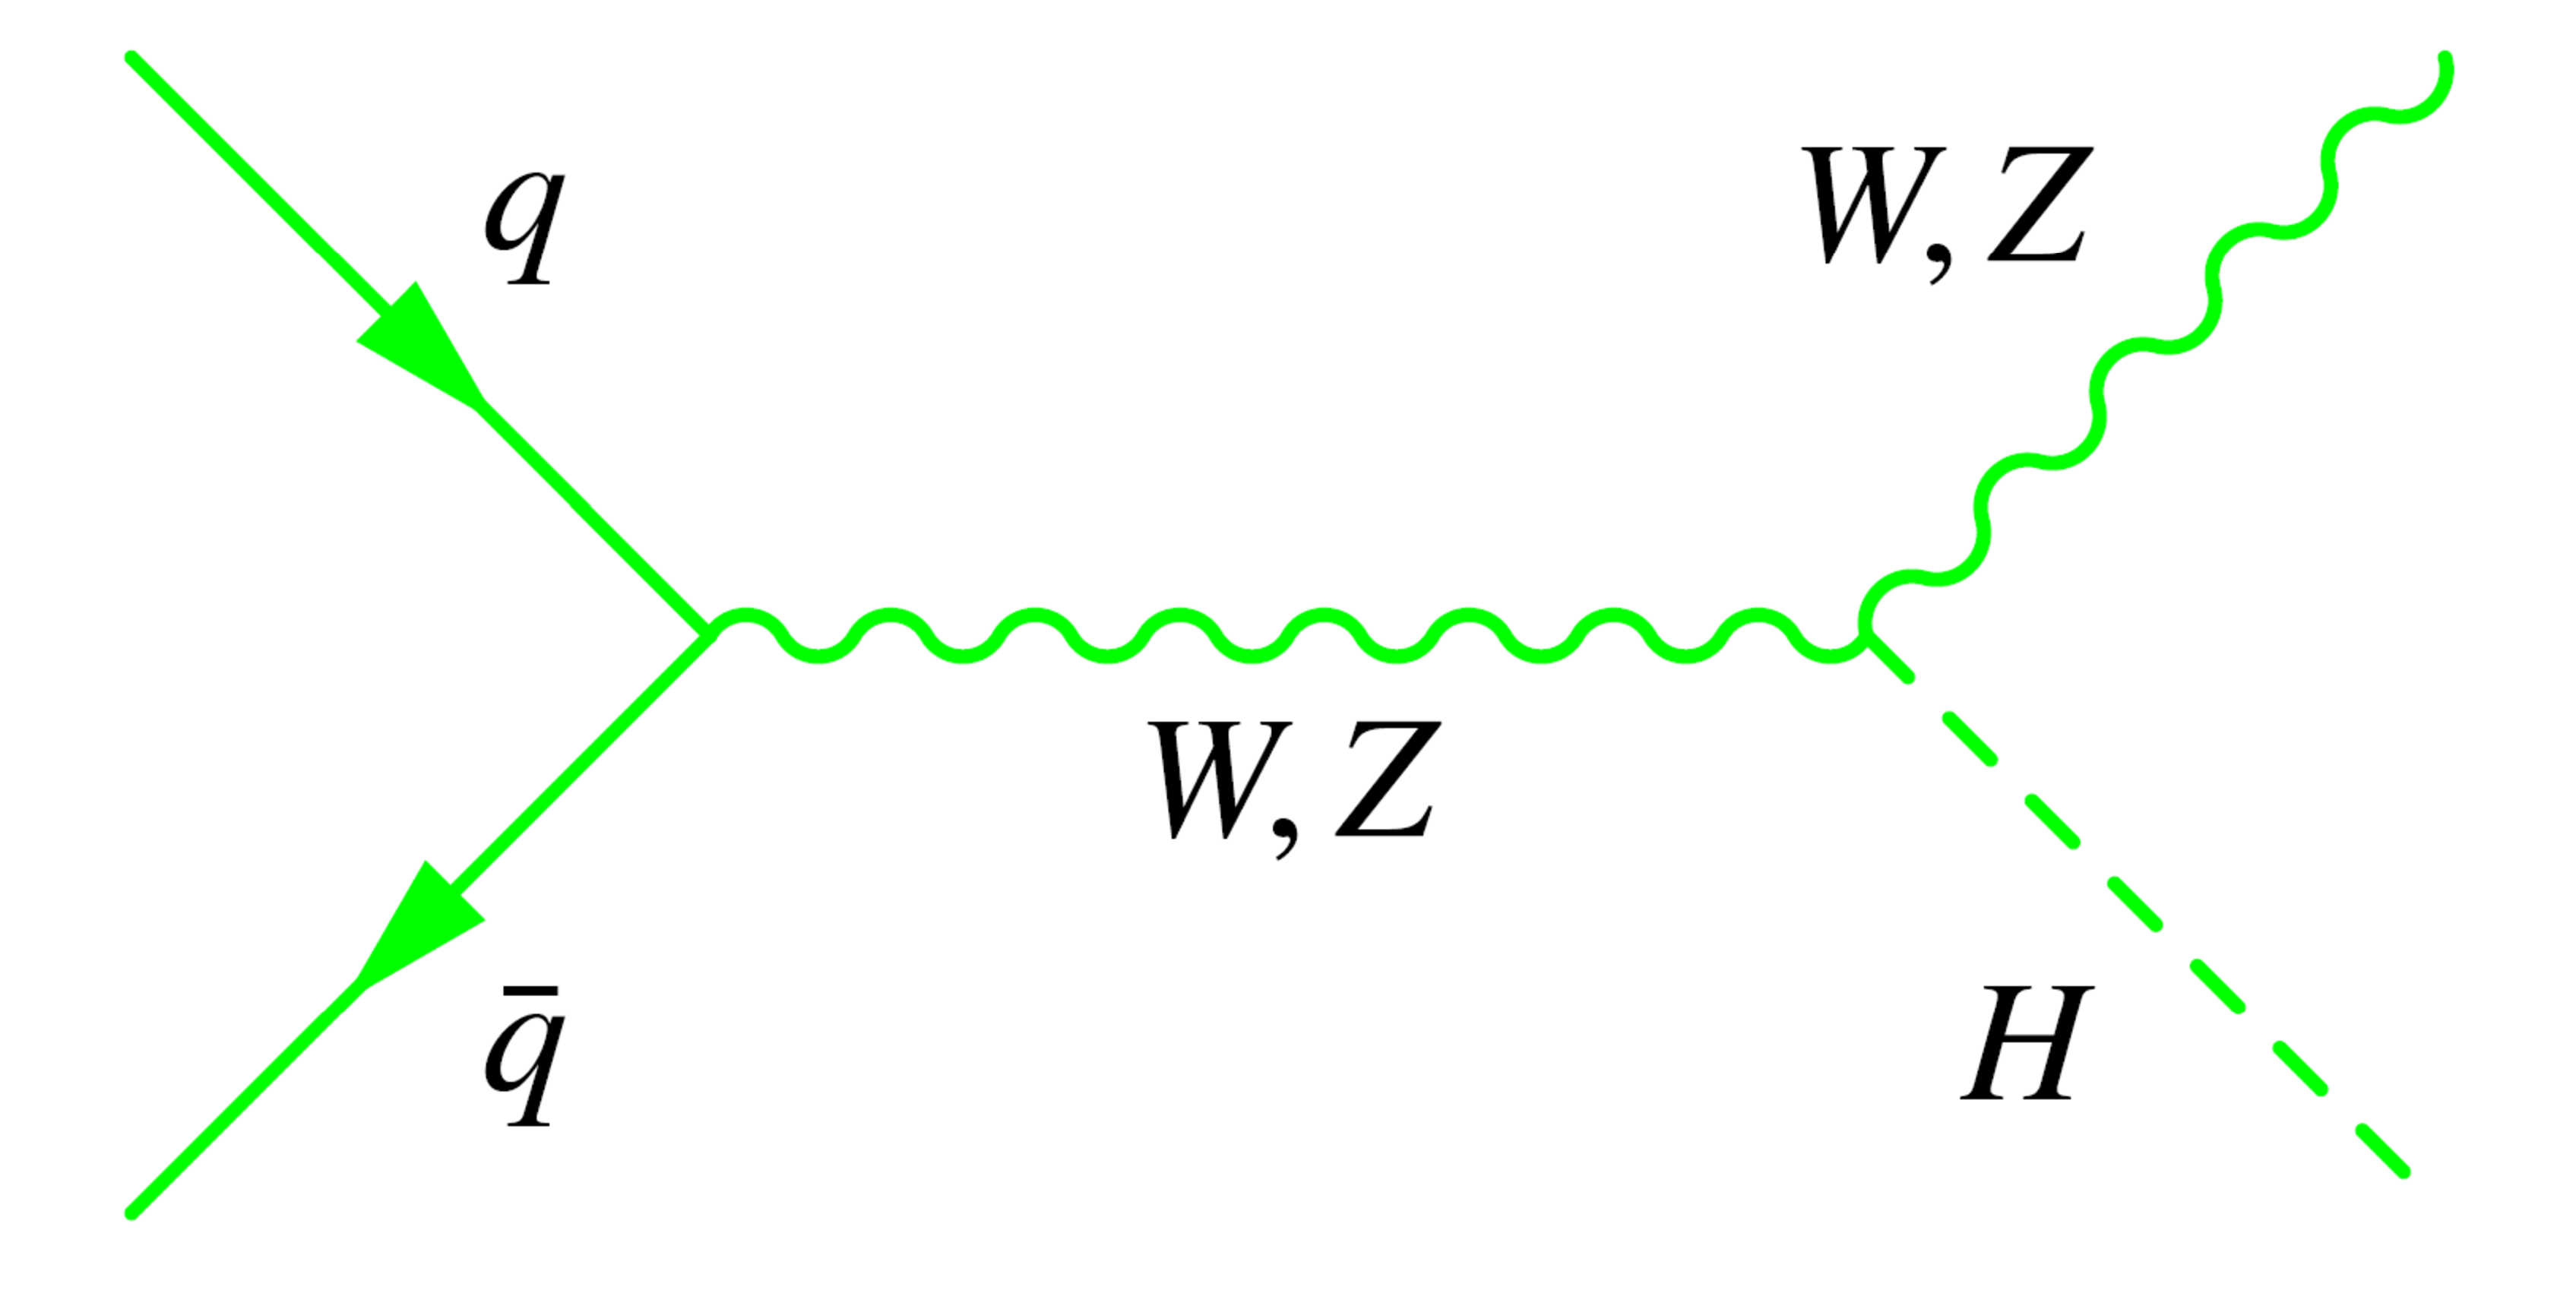
\includegraphics[width=0.45\textwidth]{images/VH.pdf}
}
\subfigure[\ttH]{
  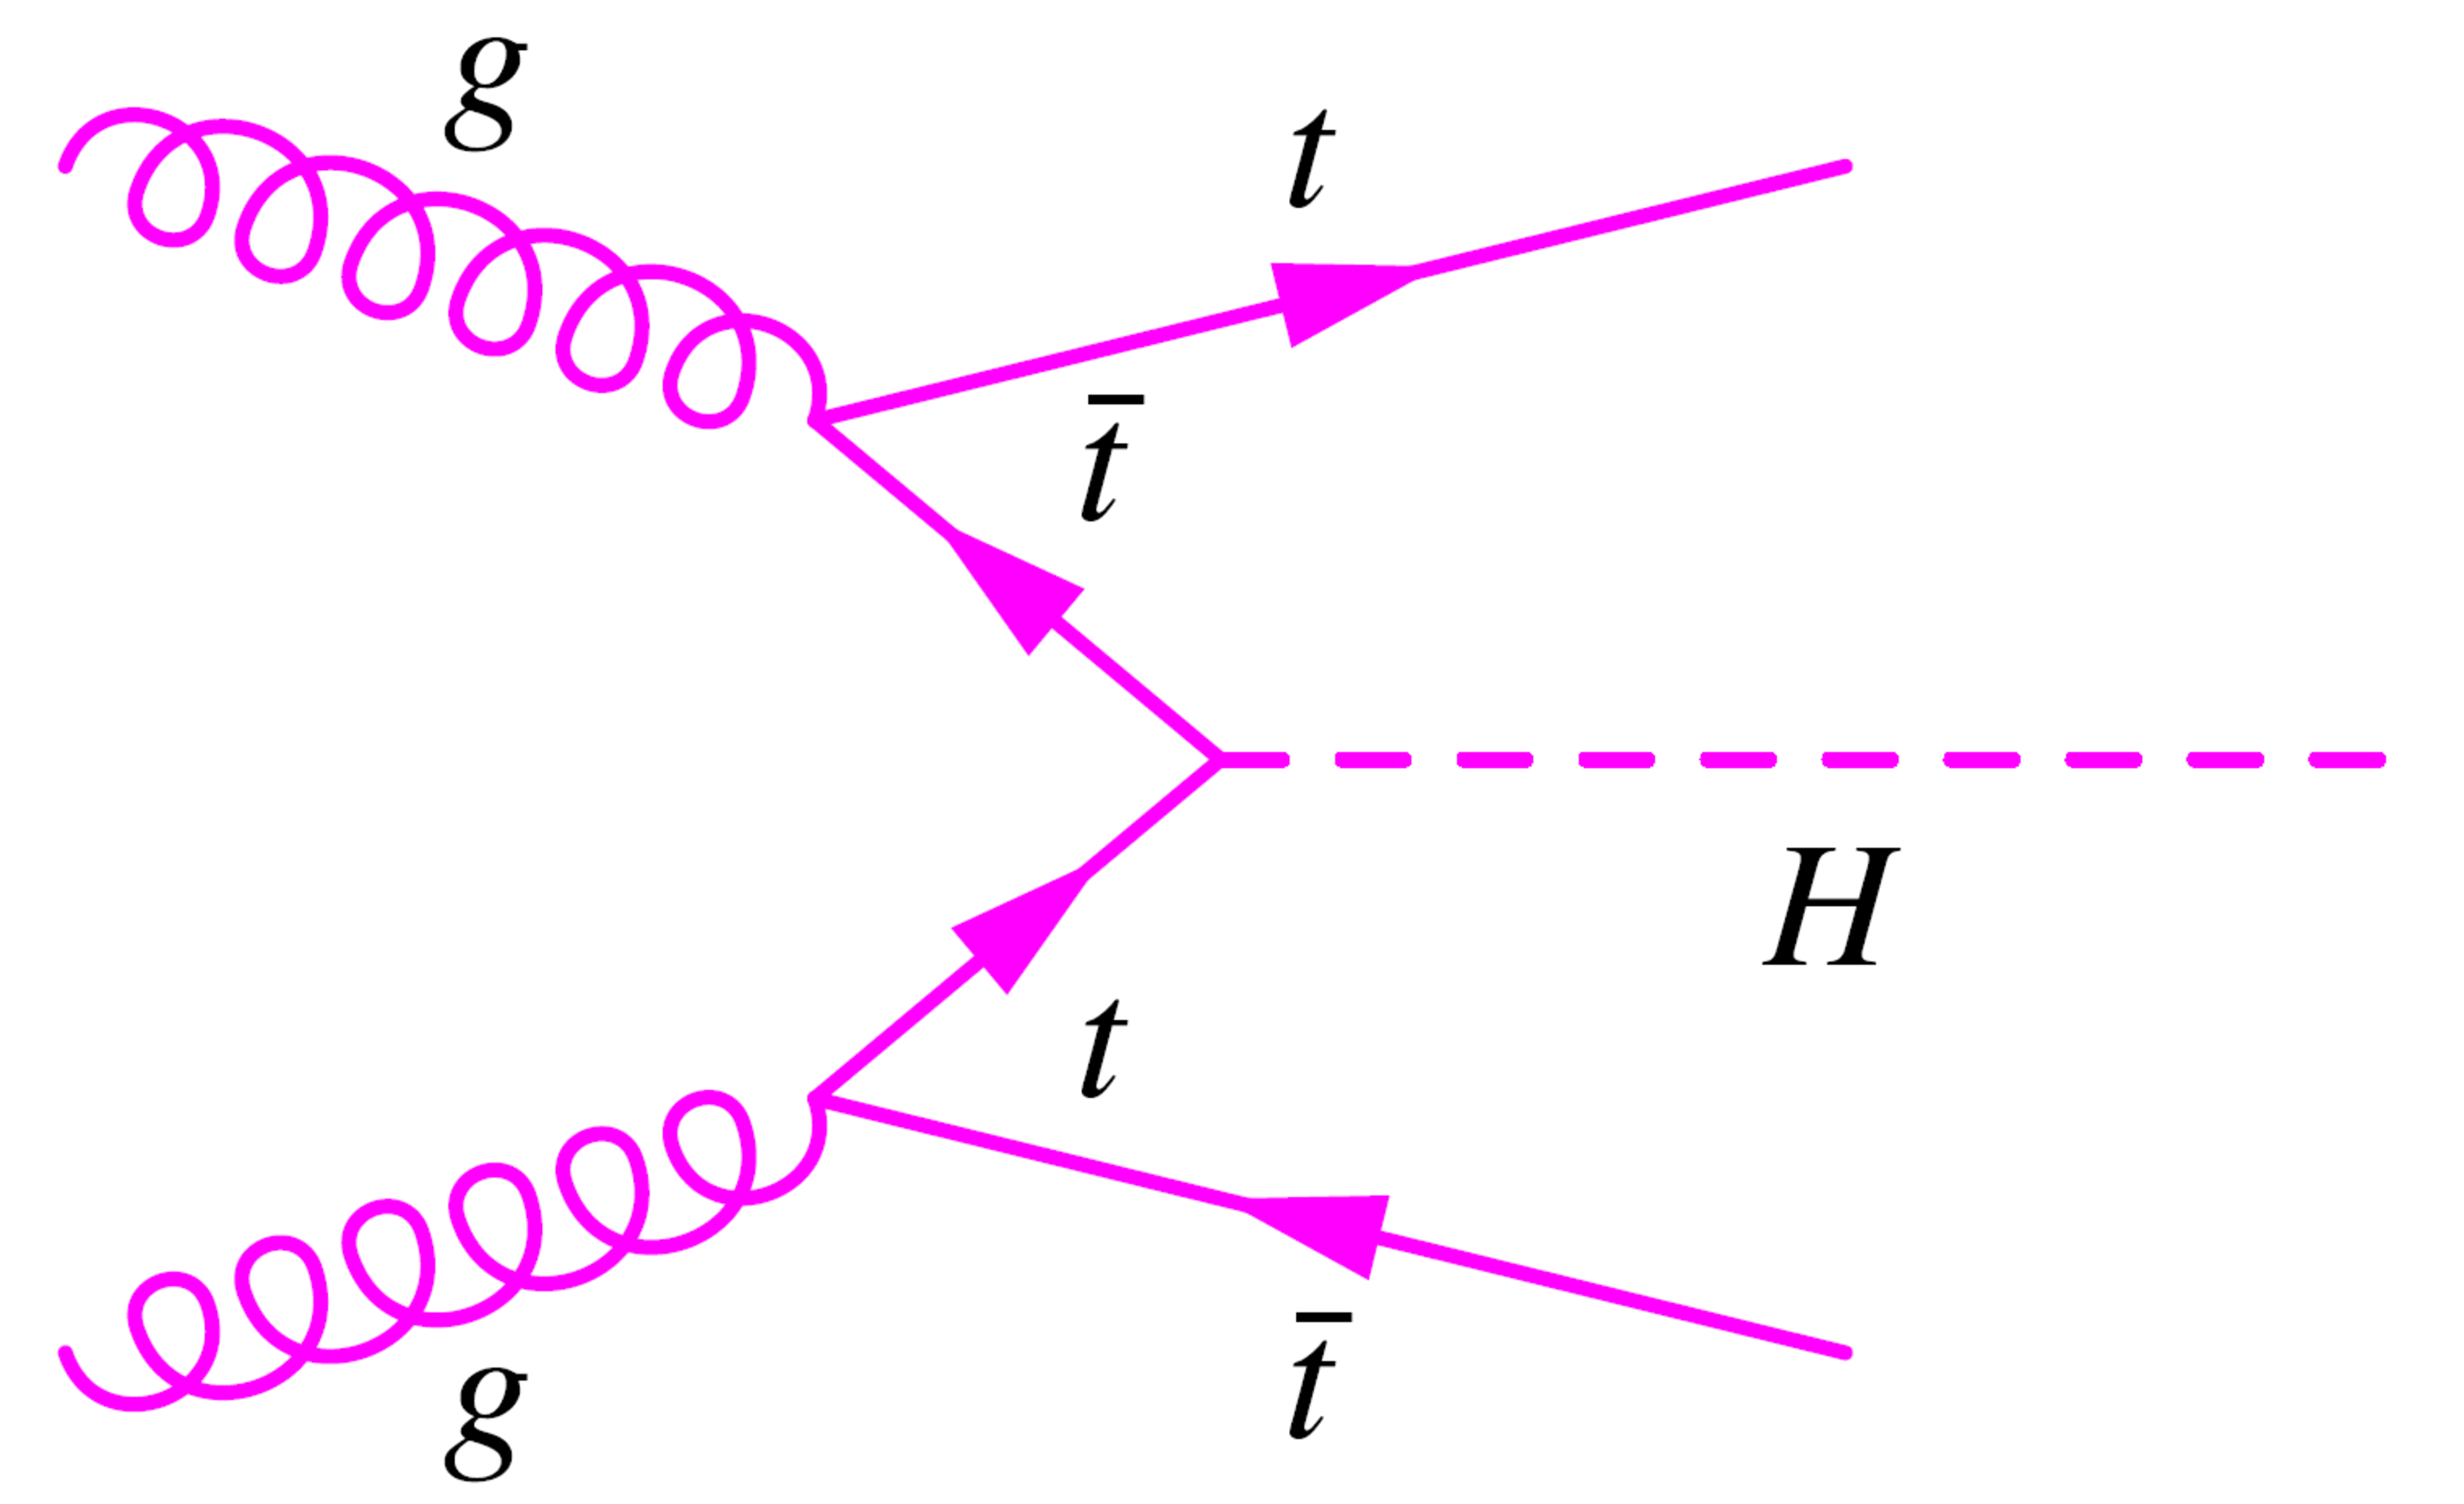
\includegraphics[width=0.45\textwidth]{images/ttH.pdf}
}
\caption{Main Higgs boson production processes at LHC.}\label{fig:higgs_prod}
\end{figure}

In order of decreasing cross section, the Higgs boson production modes are:

\begin{itemize}
\item \emph{Gluon fusion} (ggH): this is the main Higgs boson production mode at LHC over the whole mass spectrum. The process involves the fusion of two incoming gluons that give rise to the Higgs boson through a heavy quark loop, whose main contribution comes from the top quark, as shown in Fig.~\ref{fig:higgs_prod}(a).

\item \emph{Vector Boson Fusion} (VBF): each of the two interacting quarks emit a W or Z boson which, in turn, interact to produce the Higgs boson, as shown in Fig.~\ref{fig:higgs_prod}(b). Quarks deriving from the incoming partons after the emission of vector bosons proceed in the forward direction and represent the peculiar signature of this production mode, i.e. two high energy forward jets separated by a large pseudorapidity gap. This process has a cross section which is one order of magnitude lower than ggH for a large range of $m_\mathrm{H}$ values and it becomes comparable to ggH only for masses of the order of 1\TeV.

\item \emph{Vector boson associated production} (VH): also known as \emph{Higgsstrahlung}, this process is characterized by the emission of a Higgs boson from a $\mathrm{W}^\pm$ or Z boson produced by two incoming quarks, as depicted in Fig.~\ref{fig:higgs_prod}(c). The VH cross section is several orders of magnitude lower than the ggH and VBF cross sections.

\item \emph{Top quark associated production} (\ttH): a pair of top quarks, originated from the splitting of two incoming gluons, interacts to give rise to a Higgs boson, as illustrated in Fig.~\ref{fig:higgs_prod}(d).
\end{itemize}

Another production mechanism analogous to the \ttH process and with a similar cross section is the b quark associated production.

The SM Higgs boson production cross section for the various production modes depends on the Higgs boson mass and on the centre-of-mass energy, as shown in Fig.~\ref{fig:higgs_xsec}. In general, the production cross section of all processes decreases with increasing the Higgs boson mass, while the raise of the centre-of-mass energy reflects in an increase of the cross section over the whole mass range.

\begin{figure}[htb]
\centering
\subfigure{
  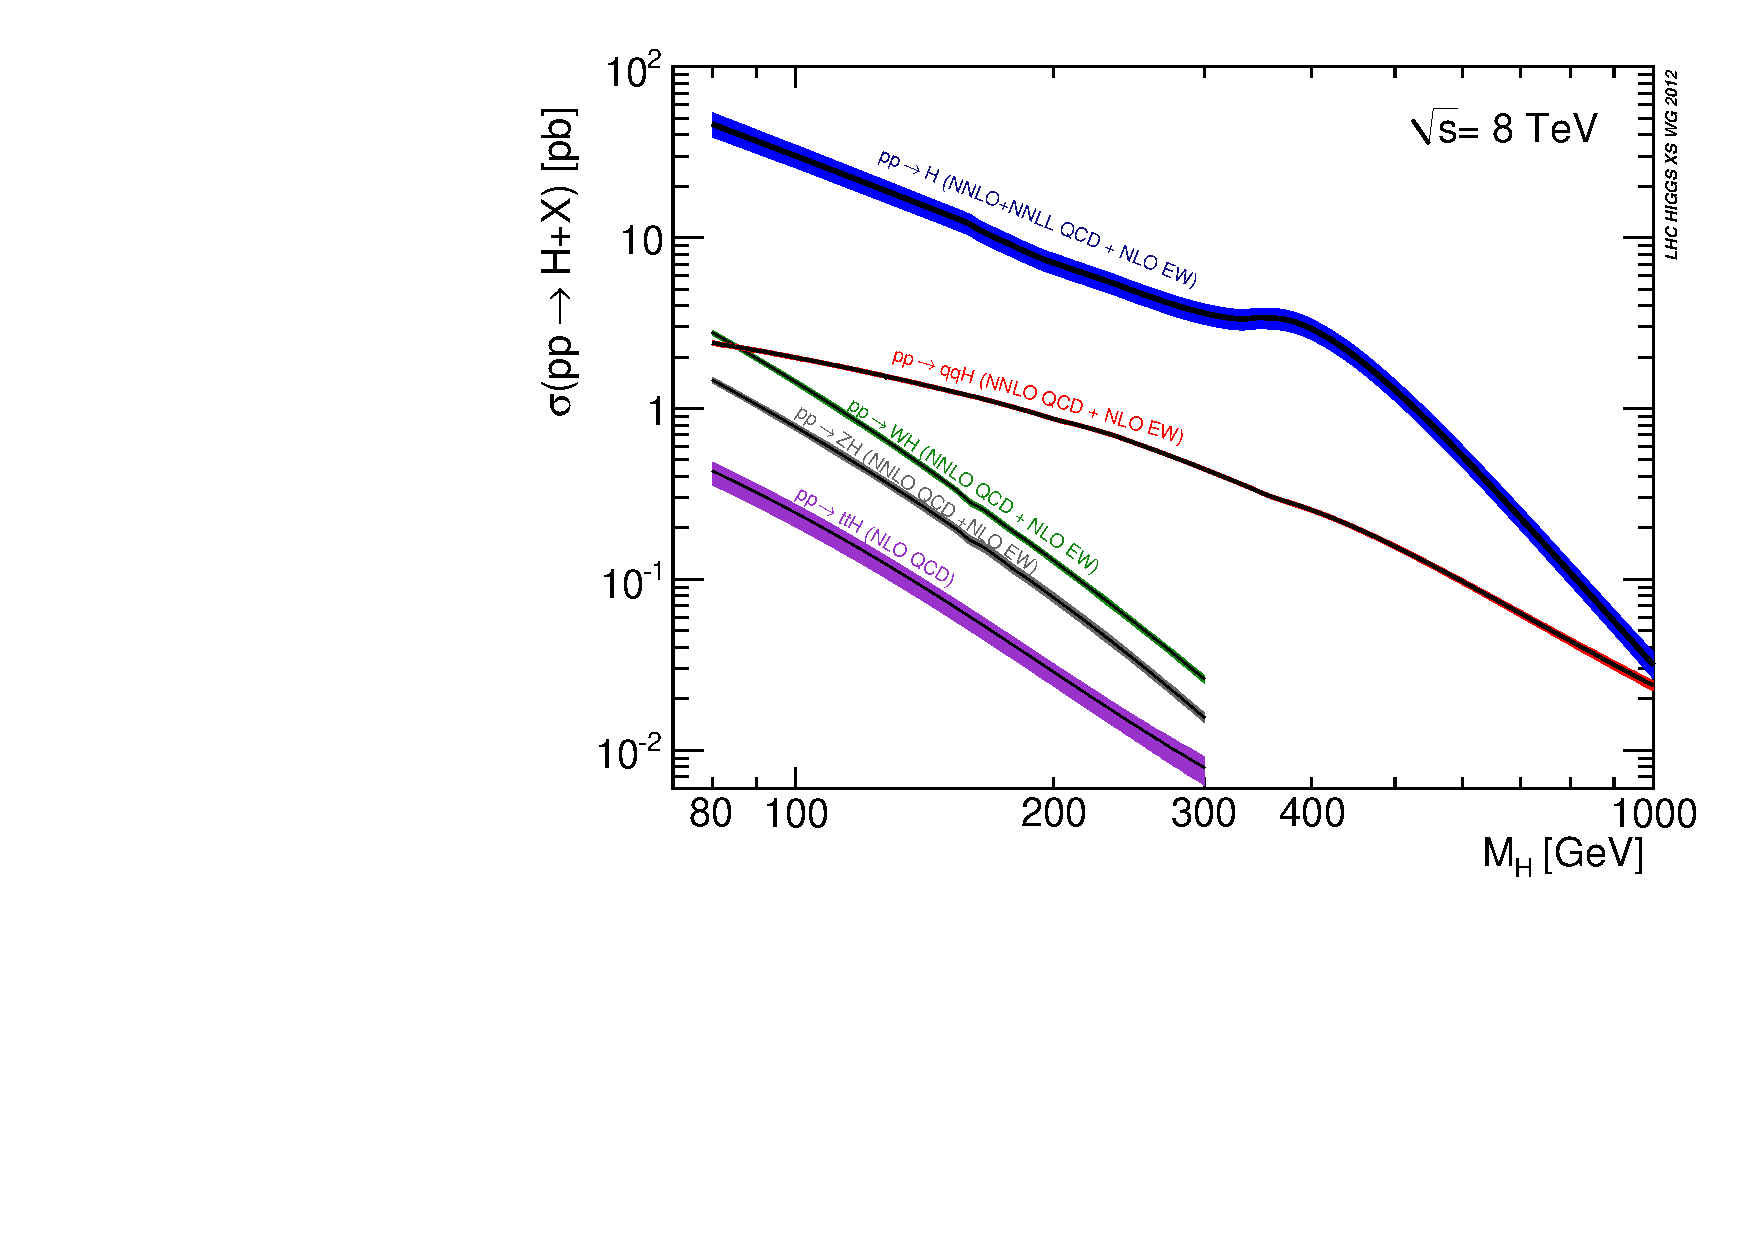
\includegraphics[width=0.45\textwidth]{images/XS_8TeV.pdf}
}
\subfigure{
  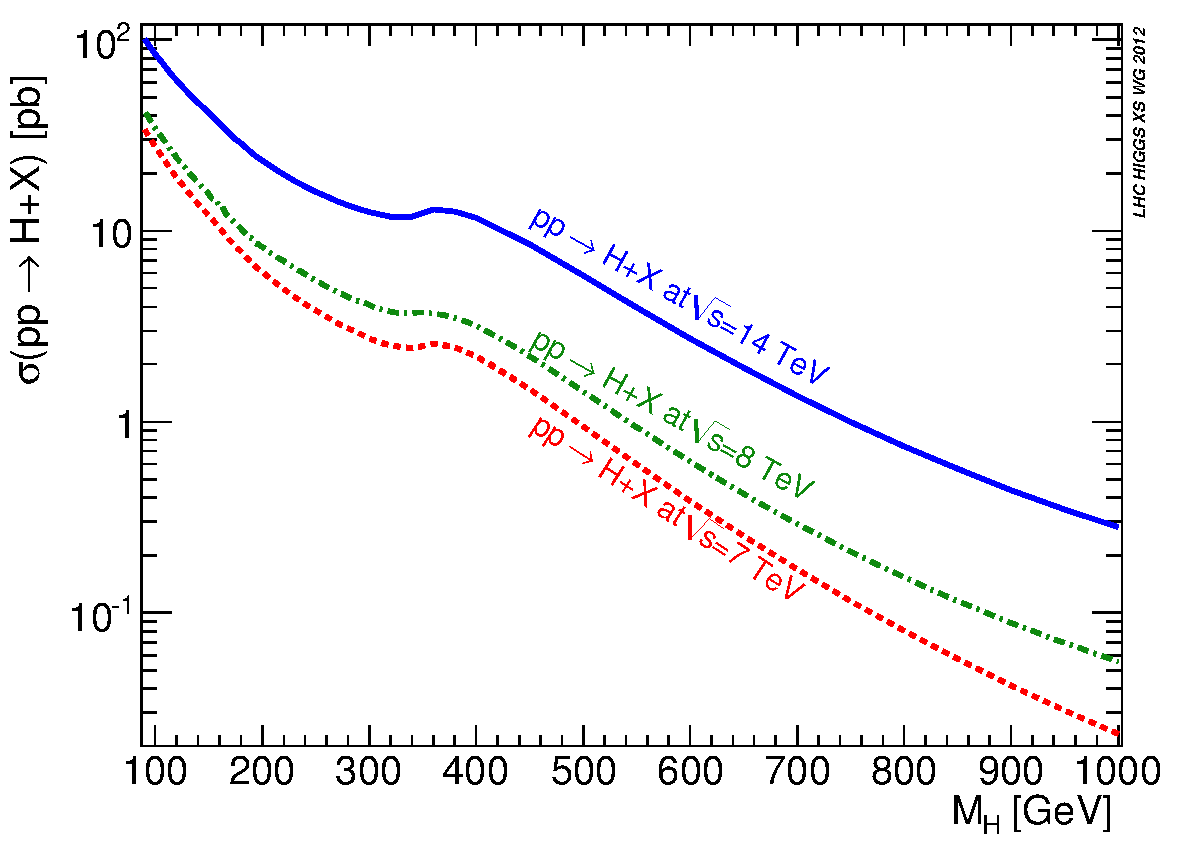
\includegraphics[width=0.45\textwidth]{images/totalXS.pdf}
}
\caption{Higgs boson cross section as a function of $m_\mathrm{H}$ for the various production mechanisms (left) and for different centre-of-mass energies (right).}\label{fig:higgs_xsec}
\end{figure}

The Higgs boson can decay to a variety of final states that can be divided in bosonic channels, like $\gamma\gamma$, ZZ or $\mathrm{W^+W^-}$, and fermionic channels, like $\tau\tau$, $b\bar b$, etc.
Its branching ratio also depends on the Higgs boson mass, as illustrated in Fig.~\ref{fig:higgs_br}, where different decay channels are compared over the whole mass spectrum.

\begin{figure}[htb]
\centering
\subfigure{
  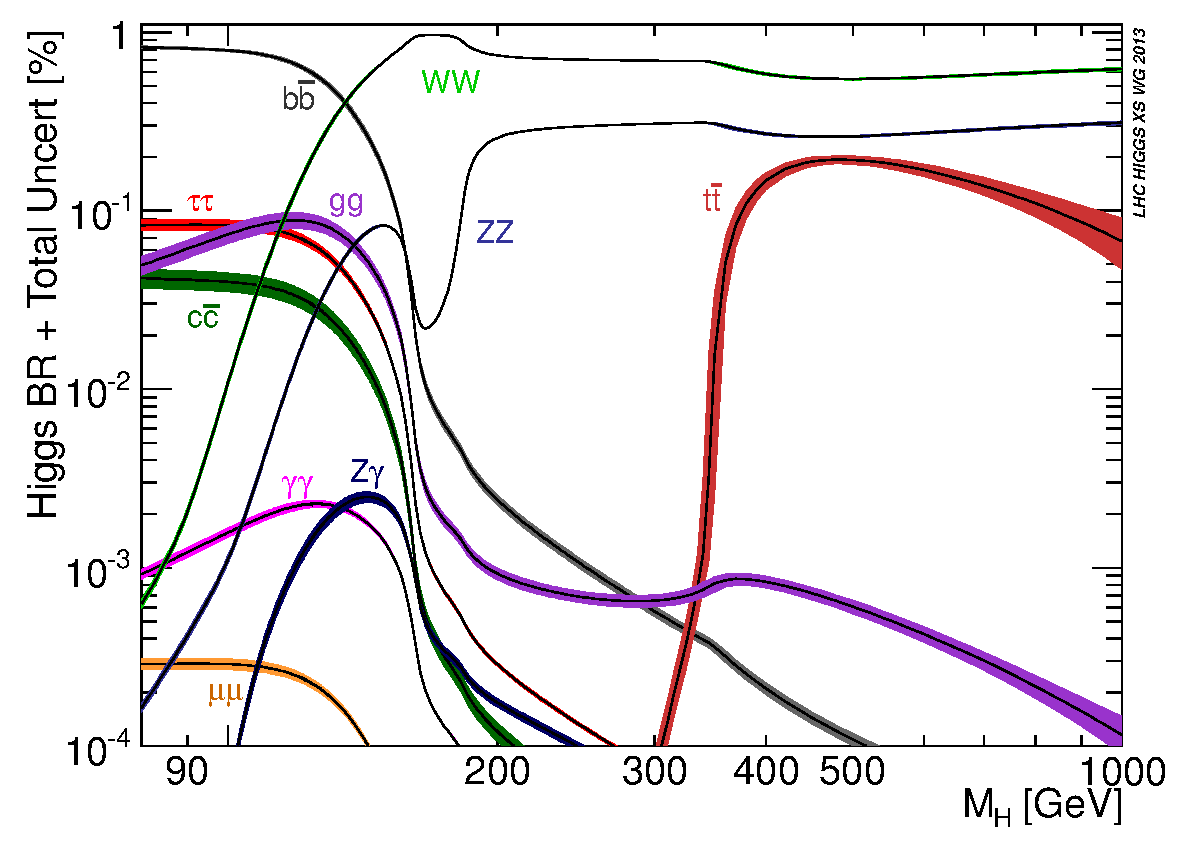
\includegraphics[width=0.45\textwidth]{images/Higgs_BR.pdf}
}
\subfigure{
  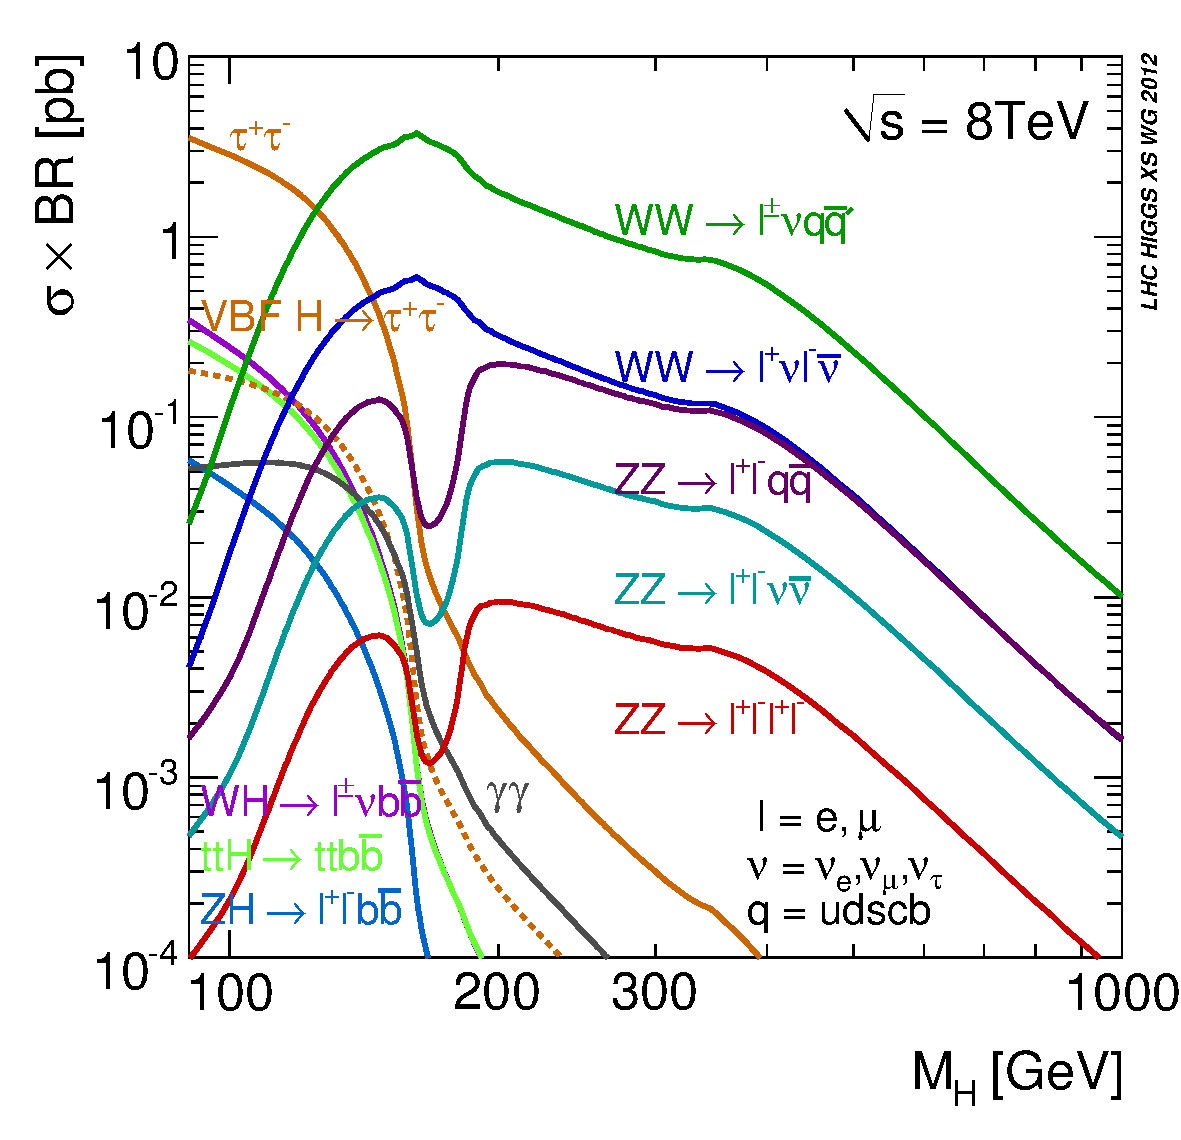
\includegraphics[width=0.45\textwidth]{images/Higgs_BR_2.pdf}
}
\caption{Higgs boson branching ratio (left) and cross section times branching ratio (right) for all the decay channels as a function of $m_\mathrm{H}$.}\label{fig:higgs_br}
\end{figure}


